\section{LiDAR}\label{sec:LiDARStateOfArt}
\noindent \paragraph{LiDAR(Light Detection And Ranging)} is an active form of remote sensing: information is obtained from a signal which is sent from a transmitter and reflected by a target and detected by a receiver back at the source. Following types of information can be obtained:
\begin{enumerate}
\item \textit{Range to target} - topographic LiDAR or laser altimeter.
\item \textit{Chemical properties of target} - differential absorption LiDAR.
\item \textit{The velocity of target} - Doppler LiDAR.
\end{enumerate}

\noindent Chemical properties of the target are out of scope. The velocity of  target seems as interesting property to investigate, but this type of LiDAR is usually used for meteorological measurements of wind currents \cite{martin2011meteorological}. Extended research in LiDAR as obstacle detection sensor has been executed by research group around Sabatini \cite{sabatini2014lidar} and Ramasy \cite{ramasamy2016lidar}. 

A LiDAR output is represented as point cloud it is described by the definition:

\begin{definition}[Scanned point and Point-cloud]
Consider viewpoint as the origin of $\R^3$ space,  Let  $point \in Polar Coordinates$ be defined as:
    \begin{equation}
        point = [ distance, horizontal^\circ, vertical^\circ, time ]^T
    \end{equation}
    Where $horizontal^\circ$ is the horizontal angle from the origin, $vertical^\circ$ is a vertical angle to the origin, and, $time$ is a time of retrieval.\\

    \noindent Point-cloud is set of points scanned in small enough time-frame, based on processing raw point data it can have following representations:
    
    \begin{enumerate}
        \item \emph{Local point-cloud} - position of the sensor is used as the origin of space and points can be represented in orthogonal or planar representation. 
        
        \item \emph{Global point-cloud} -global position of the sensor is used as a reference to calculate the global position of points.
    \end{enumerate}
\end{definition}

\paragraph{Point-cloud} is usually addressed as \textit{raw point-cloud} in case if it is represented in Local planar coordinates. Other forms of point cloud require further processing, and they are not feasible for real-time obstacle detection and avoidance \cite{chen2007airborne}.

\begin{figure}[H]
    
    \begin{subfigure}{0.45\textwidth}
        \centering
        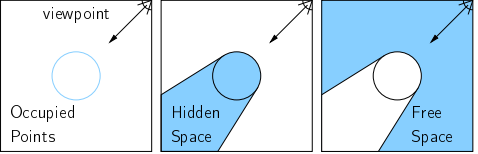
\includegraphics[width=0.9\linewidth]{\FIGDIR/10_Lidar_sets1.PNG} 
        \caption{Space type definitions}
        \label{fig:Spacetypes}
    \end{subfigure}
    \begin{subfigure}{0.45\textwidth}
        \centering
        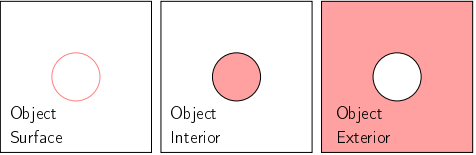
\includegraphics[width=0.9\linewidth]{\FIGDIR/11_Lidar_sets2.PNG}
        \caption{Object properties definitions}
        \label{fig:ObectProperties}
    \end{subfigure}
    
    \caption{Six space classifications \cite{yapo2008probabilistic}.}
    \label{fig:Spaces of interests}
 \end{figure}
 
\noindent  Because of real-time obstacle avoidance, it is necessary to introduce the following terminology:
\begin{enumerate}
    \item \textit{Occupied points} - points which have been detected by LiDAR (also addressed as visible points).
    \item \textit{Hidden space} - space which is hidden behind occupied points, from the viewpoint it is uncertain what is in that space. 
    \item \textit{Free space} - space which is visible from viewpoint and it is not occupied by known objects.
    \item \textit{Object surface} - detected and undetected object surface
    \item \textit{Object interior} - occupied space by the object.
    \item \textit{Object exterior} - free space around known objects.
\end{enumerate}

\noindent The existing method for space segregation \cite{yapo2008probabilistic} leads to the following definition:

\begin{definition}[Accessible space]\label{def:accessibleSpace}
    Consider known space as space explored by sensor (it can have different viewpoint along previous 3D trajectory).
    The intersection between \textit{object exterior} ($Exterior$) and \textit{free space} $Free$ gives us \textit{Accessible space} ($Accessible$).
    \begin{equation}
        Accessible = Exterior(object) \cap Free(object)
    \end{equation}
\end{definition}
 
 \noindent Accessible space $S_A$ (def. \ref{def:accessibleSpace}) is our bordering limitation for reachable space of system $ReachSet[\tau, time_0, state_0]$ (def. \ref{def:reachset01}.).